\chapter{Forret: Plus og gange}
\index{aritmetik!heltals-|textbf}\index{heltal|textbf}
\renewcommand{\labelprefix}{ch:amuse}
\llabel{}


\vspace*{-4.5cm}
\mbox{}\hspace{\fill}\includegraphics[width=3cm]{img/Al-Khwarizmi2.eps} 

\vspace{1cm}
\aufmacher{\noindent 
Forrettens funktion er at vække appetit for resten af menuen.
Det er netop formålet med dette kapitel:
For at vække læserens interesse for algoritmiske%
\footnote{Frimærket fra det tidligere Sovjetunionen viser den persisike matematiker og astronom \emph{Muhammad ibn Musa al-Chwarizmi}
\index{al-Chwarizmi, Muhammad ibn Musa|textbf} 
($^*$ omtr. 780; $\dag$ mellem 835 og 850)
fra provinsen Khorasan i området af det nuværende Usbekistan. 
Ordet »algoritme«
\index{algoritme|textbf} 
kommer fra hans navn.} 
teknikker præsenterer vi et overraskende resultat:
At folkeskolemetoden for at gange to naturlige tal
\index{multiplikation (naturlige tal)!skolemetoden} 
sammen er ikke den bedste multiplikationsalgoritme.
Der findes nemlig hurtigere metoder, hvis effektivitet gør sig gældende, når tallene bliver meget store, dvs. består af tusinder af cifre.
Vi skal betragte såden en metode i dette kapitel.} 

Aritmetik på »lange« (dvs. mangecifrede) heltal
\index{multiplikation (heltal)!anvendelse}
bruges i kryptografi, geometriske beregninger og computeralgebra.
En forbedret multiplikationsalgoritme er derfor ikke bare en intellektuelt højdepunkt, men finder også praktisk anvendelse.
Undervejs til denne algoritme skal vi -- i denne meget simple kontekst -- stifte bekendskab med nogle grundlæggende teknikker fra
algoritmekonstruktion, -analyse og -implementation.

I det følgende går vi ud fra, at naturlige tal%
\footnote{I dette kapitel betyder »tal« altid »naturligt tal«.}
% TODO: konsekvensret til naturlige tal
som sædvanligt er repræsenteret som følger af cifre.
\index{ciffer|textbf}
I et talsystem med grundtal\index{grundtal|textbf} $B$, hvor $B$ er et naturligt tal større end 1, findes cifrene $0$, $1$, $\ldots$, $B-1$, og en følge $a_{n-1}a_{n-2}\ldots a_1 a_0$ af cifre repræsenterer tallet $\sum_{0 \le i < n} a_i B^i$.
De vigtigste systemer med et lille gundtal $B$ er det binære talsystem (grundtal 2, cifrene 0 og 1), decimalsystemet (grundtal~10, cifrene 0 til 9) og det heksadecimale talsystem (grundtal~16, cifrene 0 til 15, ofte skrevet som $0$, $\ldots$ , $9$ , A, B, C, D, E, F.
Større grundtal som fx $2^8$, $2^{16}$, $2^{32}$ og $2^{64}$ forekommer også.
For eksempel repræsenterer
\begin{align*}
\text{»10101«} &\text{ i basis \phantom{0}2}&\text{værdien } & 1\cdot 2^4 + 0\cdot 2^3 + 1 \cdot 2^2 +
0 \cdot 2^1 + 1 \cdot 2^0 &= \phantom{2}21\,,\\
\text{»924«} &\text{ i basis 10}&\text{værdien }  & 9 \cdot 10^2 + 2\cdot
10^1 + 4 \cdot 10^0       &= 924\,.
\end{align*}

Vi vil gå ud fra, at vi har to elementaroperationer til rådighed:
\index{elementaroperation!heladderer} 
addition af tre cifre med et tocifret resultat (sommetider kaldt en heladderer)
\index{mente}
og multiplikationen af to cifre, ligeledes med et tocifret resultat.%
\footnote{Læg mærke til, at summen af tre cifre højest er $3(B - 1)$ og produktet af to cifre højest er $(B-1)^2$, og at begge disse tal er højest $(B-1)\cdot B^1 + (B - 1)\cdot B^0 = B^2 - 1$, og derfor kan repræsenteres med to cifre.}
I tilfældet $B=10$ gælder for eksempel
\[  \begin{array}{r} 3 \\ 5 \\ {}+{}\;\;5 \\ \hline 13 \end{array}
\qquad\text{og}\qquad    6 \cdot 7 = 42 \,. \]
Vi vil måle effektiviten naf vores algoritmer i termer af antallet af brugte elementaroperationer.

Hvert tal bestående af $n$ cifre kan man skrive med $m$ cifre for $m \ge n$ ved at foranstille nuller.
For eksempel repræsenterer »425« og »000425« samme tal. 
I det følgende går vi ud fra, at additionens eller multiplikationens operander, som vi kalder $a$ og $b$, begge består af $n$ cifre.
Antagelsen, at de to tal har samme længde, gør vores analyse nemmere, uden at vi går glip af kapitlets væsentlige indsigter.
Vi vender tilbage til denne bemærkning til sidst.
Cifrene i $a$ kalder vi $a_{n-1}$, $\ldots$, $a_0$, hvor $a_{n-1}$ er det mest betydende og $a_0$  er det mindst betydende ciffer.
%TODO højst højest lavest mest
vi skiver $a = (a_{n-1}\ldots\,a_0)$.  
Det mest betydende ciffer kan være 0.
På samme måde lader vi tallet $b$ bestå af cifrene $b_{n-1}$, $\ldots$, $b_0$ og skriver $b =(b_{n-1}\ldots\,b_0)$.


%%%%%%%%%%%%%%%%%%%%%%%%%%%%%%%%%%%%%%%%%%%%%%%%%%%%%%%%%%%%%%%%%%%%%%
\section{Addition}
\index{addition|textbf}
%%%%%%%%%%%%%%%%%%%%%%%%%%%%%%%%%%%%%%%%%%%%%%%%%%%%%%%%%%%%%%%%%%%%%%

Alle ved, hvordan man lægger
$a = (a_{n-1}\ldots\,a_0)$ og $b = (b_{n-1}\ldots\,b_0)$ sammen.
Vi skriver blot tallene under hinanden, forskudt efter de mindst betydende cifre, og lægger de enkelte cifre sammen fra højre til venstre.
Herved flyttes et enkelt ciffer fra en position til den næste.
Dette ciffer kaldes \emph{menten}. 
\index{mente}
Resultatet er et $(n+1)$-cifret tal $s=(s_n\ldots\,s_0)$.
Metoden kan fremstilles grafisk som på følgende måde:

\[       \begin{array}  {rrrrrr}
                        & a_{n-1} &\ldots &a_1 &a_0 & \text{første operand}\\
                           &b_{n-1} & \ldots &b_1  &b_0 &\qquad\qquad\text {anden operand}\\ 
                 c_n &c_{n-1} & \ldots &c_1  & 0  &\text{menter}\\ \hline
                     s_n &s_{n-1} & \ldots &s_1  &s_0  &\text{sum}\end{array} 
\]
Her er $c_0,\ldots,c_n$ følgen af menter, og $s = (s_n\ldots\,s_0)$ den resulterende sum. 
Der gælder $c_0 = 0$, $c_{i+1}\cdot B + s_i  = a_i + b_i + c_i$ for $0 \le i < n$ og $s_n = c_n$. 
Som program kan vi skrive algoritmen på følgende måde:
\begin{quote}
\begin{code}
\DeclareInit{$c$}{\Id{Ciffer}}{$0$}\RRem{Variabel for menten}\\
\ForFromTo{i}{0}{n-1} {\rm adder $a_i$, $b_i$, $c$ for at danne $s_i$ og den nye mente $c$}\\
$s_n\Is c$
\end{code}
\end{quote}

Algoritmen bruger en elementaroperation per position og derfor $n$ elementaroperationer i det hele.

\begin{thm} 
  Addition af to heltal med $n$ cifre kræver præcis $n$ elementaroperationer.
  Resultatet er et $(n+1)$-cifret tal.
\end{thm}

%%%%%%%%%%%%%%%%%%%%%%%%%%%%%%%%%%%%%%%%%%%%%%%%%%%%%%%%%%%%%%%%%%%%%%
\section{Multiplikation: Skolemetoden}
\index{Multiplikation (heltal)!skolemetode|textbf} 

Alle ved, hvordan man ganger to tal sammen.
I dette afsnit skal vi gense »skolemetoden« for multiplikation.
I et senere afsnit skal vi kigge på en anden metode, som er betydliget hurtigere for store tal.

Vi begynder langsomt.
Først skal vi forstå, hvordan man ganger et $n$-cifret tal $a$ med et etcifret tal $b_j$.
Vi bruge betegnelsen $b_j$, fordi det skal vise sig praktisk længere fremme i argumentet.
For hvert ciffer Ziffer $a_i$ i $a$ danner vi produktet $a_i \cdot b_j$.
Resultatet er et tocifret tal $(c_i d_i)$, dvs.
\[ a_i \cdot b_j = c_i \cdot B + d_i \qquad\text{for }i\in \{0,\ldots, n-1\}\,. \]
Ud fra alle cifrene $c_i$ og $d_i$ danner vi to tal $c = (c_{n-1} \ldots\, c_{0} \, 0)$ og $d = (d_{n-1} \ldots\, d_0)$.
Idet $c_i$-cifrene er højestbetydende, hægter vi et ekstra 0 på $c$.
Nu lægger vi $c$ og $d$ sammen og får produktet $p_j = a \cdot b_j$. 
Grafisk ser det ud på følgende måde:
\[ (a_{n-1} \ldots\, a_i \ldots\, a_0) \cdot b_j  \quad \longrightarrow \quad
\begin{array}{llllllll}
          c_{n-1} &  c_{n-2} & \ldots & c_{i} & c_{i-1} &\ldots &c_0 & 0  \\
                 &  d_{n-1} & \ldots  & d_{i+1} & d_{i} &\ldots &d_1 &d_0
\\ \hline 
  \multicolumn{8}{c}{\text{Summen af $c$ og $d$}}
\end{array}
\]
Hvor mange elementaroperationer har vi brugt?
For hvert $i\in\{0,\ldots, n-1\}$ kræves en elementaroperation for at danne produktet $a_i \cdot b_j$.
For at lægge $(c_{n-1}\ldots c_0\,0)$ og $(d_{n-1}\ldots d_0)$ kan vi nøjes med at kopiere $d_0$ uden at betale nogen operation, de andre position kræver en elementaraddition.
Total giver det $2n$ elementaroperationer.
Læg mærke til, at mente i den sidste elementaraddition er $0$, fordi $a\cdot b_j \le  (B^n-1)(B-1) < B^{n+1}$.
Resultatet består altså af $n+1$ cifre.

\begin{lemma} 
  Multiplikation af et $n$-cifret og et etcifret tal kan gøres med $2n$ elementaroperationer.
  Resultatet er et $(n + 1)$-cifret tal.
\end{lemma}

I praksis vil man nok være lidt mere snedig.
Man sammenfatter nemlig dannelsen af cifferprodukutet $a_i \cdot b_j$ og additionen af $c$ og $d$ i samme fase,
\footnote{I oversætterkonstruktion
\index{oversætter}
\index{løkkefusion} 
kaldes denne transformation, som hører til kodegenerering og kodeoptimering, for \emph{løkkefusion}.} 
dvs. at de enelte cifre i $c$ og $d$ skabes i det øjeblik, hvor de skal bruges i den afsluttende addition.
Vores algoritme danner i stedet samtlige cifferprodukter $a_i \cdot b_j$ for $i\in\{0,\ldots, n-1\}$ i en fase for sig.
Det tjener kun til at gøre beskrivelsen mere klar.

\begin{exerc} 
  Skriv et program, der ganger $a$ og $b_j$ i samme fase.
\end{exerc}

Nu er vi parate til at gange to $n$-cifrede tal.
Skolemetoden for denne opgave ser ud på følgende måde:
Vi danner delprodukterne $p_j$ (med repræsentationen $(p_{j,n}\ldots\, p_{j,0})$), ved at gange  $a$  med det $j$te ciffer $b_j$ i $b$, og adderer derefter produkterne $p_j \cdot B^j$, passende forskudt under hinanden, for at danne produktet af $a$ og $b$.
Grafiskt ser det sådan ud:
\[
\begin{array}{llllllllll}
      &   &        &            &  p_{0,n} & p_{0,n-1} &\ldots & p_{0,2} & p_{0,1} & p_{0,0} \\
      &    &       &  p_{1,n} & p_{1,n-1} & p_{1,n-2}&\ldots & p_{1,1} & p_{1,0} \\ 
& & p_{2,n} & p_{2,n-1} & p_{2,n-2} & p_{2,n-3}&\ldots & p_{2,0} \\
          &           &           & &\ldots & & \\ 
p_{n-1,n} & \ldots & p_{n-1,3} & p_{n-1,2} & p_{n-1,1} & p_{n-1,0} \\ \hline 
\multicolumn{8}{c}{\text{Summen af  de $n$ delprodukter}}
\end{array} \]
Beskrivelsen i pseudokode er vældig kompakt.
Vi initialiserer produktet $p$  til 0  og lægger delprodukterne $a \cdot b_j \cdot B^j$ til $p$ et efter et for $j\in \{0,\ldots, n-1\}$:

\begin{quote}
  \begin{code}
\DeclareInit{$p$}{$\mathbf N$}{$0$}\\
\ForFromTo{j}{0}{n-1} $p\Is p + a \cdot b_j \cdot B^j$
  \end{code}
\end{quote}

\index{algoritmenanalyse!sum}%
Nu skal vi bestemme, hvor mange elementaroperationer skolemetoden bruger.
For hvert delprodukt $p_j$ bruges $2n$ elementaroperationer, og derfor kræver beregningen af samtlige delprodukter $2n^2$ elementaroperationer i det hele.
Prouktet $a \cdot b$ består  af  $2n$ cifre, og derfor behandler hver addition $p + a \cdot b_j \cdot B^j$ tal bestående af højst $2n$ cifre.
Hver af disse $n-1$ additioner koster højst $2n$ elementaroperationer, sammenlagt højst $2n^2-2n$ mange.
I det hele bruges altså højst $4n^2$ elementaroperationer.     

En enkel observation tillader os at forbedre denne øvre grænse.
Tallet $a \cdot b_j \cdot B^j$ består af $n + 1 + j$ cifre, hvoraf de sidste $j$ har værdien 0.
Vi kan altså begynde med additionen på position $(j + 1)$.
Desuden gælder der i  det øjeblik, som $a \cdot b_j \cdot B^j$ lægges til $p$, at $p$ har værdien $a\cdot(b_{j-1}\ldots\,b_0)$, som består af højst $n+j$ cifre.
Derfor går additionen af  $p$ og $a \cdot b_j\cdot B^j$ ud på att lægge to $(n+1)$-cifrede tal sammen til et  $(n+1)$-cifret resultat, hvilket kun behøver $n + 1$ elementaroperationer. 
Sammenlagt behøver alle $n-1$ additioner ikke mere end $(n-1)(n+1) < n^2$ elementaroperationer.
Vi får følgende resultat:

\begin{thm}
  \llabel{thm:eff of school method}
  Skolemetoden udregner produktet af to $n$-cifrede tal ved brug af højst $3n^2$ elementaroperationer.
\end{thm}

Vi har analyseret antallet af elementaroperationer for addition of multiplikation med skolemetoden.
Lad $M_n$ betegne antallet af elementaroperationer, som skolemetoden bruger til multiplikation af to $n$-cifrede tal.
Vi har vist, at $M_n$ er omtrent $3n^2$.
Vi vil sige at »$M_n$ vokser \emph{kvadratisk}«.
Læg mærke til, at 
\[ \frac{M_n}{M_{n/2}} = \frac{3 n^2}{3 (n/2)^2} =  4 \,.\]
Kvadratisk vækst betyder altså, at antallet af elementaroperationer i alt væsentligt bliver 4 gange større, hver gang størrelsen af probleminstansen
\index{probleminstans}
\index{instans} 
fordobles. 


\begin{figure}[t]
\begin{minipage}[t]{0.35\textwidth}
  \begin{tabular}{S[table-format=6.0]S[table-format= 3.8]S[table-format=1.2, round-mode=places,round-precision=2]}\toprule
    {$n$} & {$T_n$ (sek.)}  & {$T_n/T_{n/2}$} \\\midrule
    8     &   0.00000469  &  \\ 
    16    &   0.0000154         & 3.28527 \\ 
    32      & 0.0000567         & 3.67967 \\ 
    64      & 0.000222          & 3.91413 \\ 
    128     & 0.000860          & 3.87532 \\ 
    256     & 0.00347           & 4.03819 \\ 
    512     & 0.0138            & 3.98466 \\ 
    1024    & 0.0547            & 3.95623 \\ 
    2048    & 0.220           & 4.01923 \\ 
    4096    & 0.880             & 4 \\ 
    8192    & 3.53              & 4.01136 \\ 
    16384   & 14.2              & 4.01416 \\ 
    32768   & 56.7              & 4.00212 \\ 
    65536   & 227               & 4.00635 \\ 
    131072  & 910               & 4.00449 \\ \bottomrule
\end{tabular}
\end{minipage}
%
  \begin{minipage}{0.65\textwidth}
    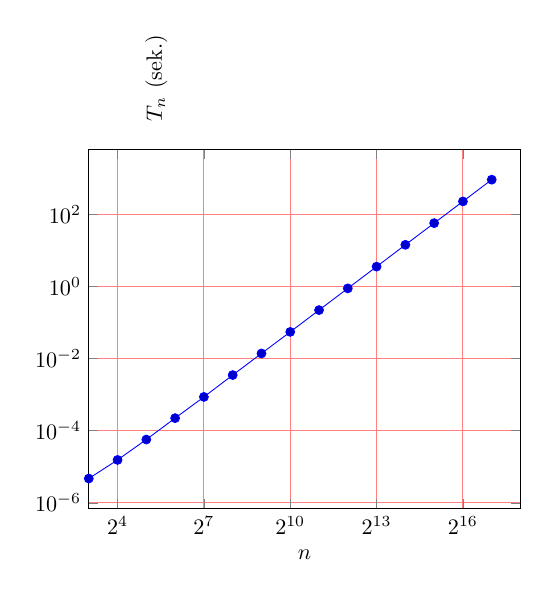
\begin{tikzpicture}[scale = .8]
    \begin{loglogaxis} [ xlabel=$n$, xmin = 8, xmax = 262144,ylabel=$T_n$ (sek.),   log basis x={2},     grid=both,
        y label style = { at = {(0.2,1.2)}, anchor = south},
      major grid style={red!50}]
	\addplot table[x=n,y=time] {
	  n time
    8        0.00000469 
    16       0.0000154  
    32       0.0000567  
    64       0.000222   
    128      0.000860   
    256      0.00347    
    512      0.0138     
    1024     0.0547     
    2048     0.220      
    4096     0.880      
    8192     3.53       
    16384    14.2       
    32768    56.7       
    65536    227        
    131072   910        
	};
	\end{loglogaxis}
\end{tikzpicture}
\end{minipage}
\caption{Udførelsestiden for skolemetoden til multiplikation af to $n$-cifrede tal.
De tre søjler i tabllen til \emph{venstre} angiver $n$, udførelsestiden $T_n$ af \protect\CC-implementationen fra afsnit~\lref{s: programs}  og forholdet $T_n/T_{n/2}$.  
Grafen til \emph{højre} tegner $\log T_n$ som funktion af $\log n$; stort set som en ret linje.
Læg mærke til, at når $T_n = \alpha n^\beta$ for konstante faktorer $\alpha$ og $\beta$, så gælder $T_n/T_{n/2} =
2^\beta$ og $\log T_n = \beta \log n + \log \alpha$.
Med anndre ord er $\log T_n$ en lineær funktion af  $\log n$ med hældning $\beta$.
I vores tilfælde er hældningen 2, hvilket man kan efterprøve med en lineal.}
\llabel{fig:school_times}
\end{figure}

Antag nu, at vi implementerer multiplikationsalgoritmen i vores yndlingsprogrammeringssprog (det gør vi faktisk forneden) og måler den tid, det tager på vores yndlingscomputer at gange par $n$-cifrede tal $a$ og $b$ for forskellige $n$.
Hvile udførelsestider kan vi regne med?
Vi påstår, at eksperimentet vil vise kvadratisk vækst i $n$.
Grunden hertil er, at \emph{elementaroperationerne er repræsentative for programmets udførelsetid}.
Betragt hertil først additionen af to $n$-cifrede tal.
Hvad sker der under programmets udførelse?
For hver cifferposition $i$ flyttes cifrene $a_i$ og $b_i$ fra hovedlageret til processoren, summen $a_i+b_i+c$ bliver regnet ud, sumcifret $s_i$ kopieres over i hovedlageret, menten $c$ aktualiseres, index $i$ tælles op og løkkeafslutningsbetingelsen prøves.
I vores analyse har vi talt præcis 1 elementaroperation for hvert $i$, derfor er antallet af elementaroperationer repræsentativt for antallet af udførte maskincykler.
På en moderne processor opstår desuden særlige fænomener som pipelining af operationer
\index{pipelining}
% TODO pipelining
og den meget vanskelige mekanisme for datastransport mellem hovelageret og processoren, men disse påvirker alle cifferpositioner nogenlunde lige.
Derfor er antallet af elementaroperationer også repræsentativt for udførelsestiden af en faktisk implementation på en virkelig computer.
Samme overvejelser kan gennemføres for multiplikationsalgoritmen, forde etcifret multiplikation ligner etcifret addition, og skolemetodens anden fase går ud på en følge af additioner.

\index{ingeniørsaspekter}%

Vi vil nu udsætte disse overvejelser for et eksperiment.
I figur~\lref{fig:school_times} vises udførelsestiderne for en \CC-implementation af skolemetoden;
programmet findes i afsnit~\lref{s: programs}.
For hvert $n$ har vi gennemført vældigt mange
\footnote{Det ur, som bruges til at måle cpu-tiden, leverer sit svar i en vis enhed, fx millisekunder, og den nødvendige afrundingsfejl medfører en fejl på op til halvdelen af enheden. 
Eksperimentet skal derfor vare meget længere en denne enhed for begrænse effekten  af denne afrundingsfejl.}
multiplikationer af tilfældige $n$-cifrede tal for at bestemme den gennemsnitlige udførelsestid $T_n$.
Denne finder man i tabellens anden søjle.
Figur~\lref{fig:school_times} viser desuden datapunkterne grafisk.%	
\footnote{I denne bog angiver $\log x$ logaritmen af $x$ med grundtal~2, altså $\log_2 x$.}%
Målepunkterne indikerer kvadratisk vækst, hvilket man kan aflæse på forskellige måder.
Forholdet $T_n/T_{n/2}$ er altid tæt på 4, og tegningen i dobbeltlogaritmisk skala viser stort set et ret linje med hældning~2.
Eksperimentet er altså ganske lovende:
\emph{Vores teoretiske analyse tillader forudsigelser af algoritmens faktiske opførsel.
Analysen kom frem til, at antallet af elementaroperationer vokser kvadratisk, vis har argumenteret for, at udførelsestiden burde ligge tæt op ad antallet af elementaroperationer, og den målte udførelsestid vokser vitterligt kvadratisk.} 
Alligevel observerer vi også systematiske afvigelser.
For små $n$ vokser tiden fra en række i tabellen til den næste med mindre end en faktor $4$.
Det hænger sammenn med, at lineære og konstante termer stadig spiller en betragtelig rolle for udførelsestiden.
For større $n$ er forholdet meget tæt på 4.
For meget store $n$ (så store, at det bliver vanskeligt at bestemme udførelsestiden eksperimentelt) ville forholdet nok blive større end $4$, fordi lageradgangstiden afhænger af størrelsen af datamængden.
Vi vender tilbage til dette punkt i afsnit~\ref{ch:intro:s:model}.

\begin{exerc} 
  Skriv programmer for addition og multiplikation af lange tal.
  Antag, at tallene er givet som følger (rækker eller lister eller hvad dit programmeringssprog nu måtte bruge af datastrukturer) af decimalcifre, og anvend den forhåndenværende aritmetik fro at implementere elementaroperationerne.
  Skriv så funktioner \texttt{plus}, \texttt{gange1} og \texttt{gange} til henholdsvis addition af to tal, multiplikation af et tal med et etcifret tal og multiplkation af $n$-cifrede tal.
  Lav din egen udgave af figur~\lref{fig:school_times}.
  Prøv også at bruge et større grundtal end 10, fx $2^{16}$.  
\end{exerc}


\begin{exerc} 
  Beskriv og analyser skolemetoden for division
  \index{division (naturlige tal)}
  af to naturlige tal. 
\end{exerc}

%%%%%%%%%%%%%%%%%%%%%%%%%%%%%%%%%%%%%%%%%%%%%%%%%%%%%%%%%%%%%%%%%%%%%%%%%%%%%%%%%%%%%%%%%%
\section{Resultatkontrol}
\index{algoritmekonstruktion!resultatkontroll}
%%%%%%%%%%%%%%%%%%%%%%%%%%%%%%%%%%%%%%%%%%%%%%%%%%%%%%%%%%%%%%%%%%%%%%%%%%%%%%%%%%%%%%%%%%

Vores additions- og multiplkationsalgoritmer er temmelig simple, så vi kan trygt gå ud fra at være i stand til at implementere dem korrekt i det valgte programmeringssprog.
Alligevel er konstruktionen af programmer kendt for at være behæftet med fejl,%
\footnote{Fejlen i divisionsalgoritmen i Pentium-processorens divisionsalgoritme for kommatal var notorisk.
Den var resultatet af en enkelt fejlagtig indgang i en tabel i algoritmen.
}
så vi bør altid interessere os for metoder for at efterprøve resultatet af en beregning.
For multiplikation lærte forfatterne i grundskolen følgende metode, som kaldes »ni-prøve«
\index{niprøve} 
(på engelsk »\emph{casting out nines}«,  på fransk »\emph{preuve par neuf}«.)

Find tværsummen af $a$, dvs. summen af de enkelte cifre.
\index{tværsum}
Hvis tværsummen har mere end et ciffer, tag tværsummen af tværsummen.
Gentag, indtil der kun er et ciffer tilbage, kaldt \emph{prøvesummen}
\index{przvesum@prøvesum} af $a$ og betegnet $s_a$.
Her er et eksempel:
\[ 4528 \rightarrow 19 \rightarrow 10 \rightarrow 1 \,.\]
Gør ligeså med $b$ og $c$ for at skabe prøvesummerne $s_b$ og $s_c$.
Beregn nu produktet $s_a \cdot s_b$ og dets prøvesum $s$.
Hvis $s$ og $s_c$ er forskellige, så er $c$ ikke produktet $a\cdot b$.
Denne prøve blev beskrevet af al-Chwarizmi\index{al-Chwarizmi, Muhammad ibn Musa} i sin algebrabog.

Lad os gennemføre niprøven på et enkelt eksempel. 
Givet $a = 429$, $b = 357$ og $c = 154153$.
Da gælder $s_a = 6$, $s_b = 6$ og $s_c = 1$. 
Endivedere er $s_a \cdot s_b = 36$ og derfor $s = 9$.
Derfor har vi $s_c \not= s$, så $c$ kan ikke være produktet af $a$ og $b$, som nemlig er $c' = 153153$. 
Prøvesummen af $c'$ er $9$, så det består niprøven.
Prøven er finder nogle, men selvfølgeligt ikke alle fejl, fx bestås den af $135153$.

For at forstå den matematiske baggrund, betragter vi en mere generel metode.
Betragt et positivt heltal $q$ (niprøven er tilfældet $q=9$).
Lad $s_a$ være resten ved heltalsdivision af $a$ med $q$ $a$ durch $q$, dvs. $s_a = a - \floor{a/q}\cdot q$.
Da gælder $0 \le s_a < q$.
I matematisk notation skriver man dette som $s_a = a \bmod q$\index{modulo}.% 
\footnote{Den metode, man måske har lært i skolen, bruger rester i området 
$1$, $\ldots$, $9$ i stedet for $0$, $\ldots$, $8$;
svarende til formlen $s_a = a - (\ceil{a/q} - 1) \cdot q$.}  
På tilsvarende måde gælder $s_b = b \bmod q$ og $s_c = c \bmod q$.
Endelig er $s = (s_a \cdot s_b) \bmod q$.
Hvis der gælder $c = a \cdot b$, så må der også gælde $s=s_c$.
Derfor medfører $s\not=s_c$, at $c\not=a\cdot b$, hvilket afslører en fejl ved multiplikationen (eller niprøven). 
Hvad ved vi, når $s = s_c$ gælder?
I så fald må $q$ dele differencen mellem  $c$ og $a \cdot b$.
Hvis denne difference ikke er $0$, opdages fejlen af hvert $q$, som ikke deler differencen.

I vores eksempel forsøger vi nu med $q=7$.
Da gælder  $a \bmod 7 = 2$ og
$b \bmod 7 = 0$, og derfor  $s = (2 \cdot 0) \bmod 7 = 0$. 
Men $135153 \bmod 7 = 4$, og vi har opdatet, at $135153$ og $429 \cdot 357$ er forskellige. 

\begin{exerc}
  Forklar, hvorfor den niprøve, forfatterne lærte i skolen, svarer til $q = 9$.
\emph{Vink}: $10^{k} \bmod 9 = 1$ for alle $k \ge 0$. 
\end{exerc}

\begin{exerc}[\emph{Elleveprøve}] 
  Det er nemt at finde resten modulo 11 af tipotenser:
  Der gælder nemlig $10^k \bmod 11 = (-1)^k$ for alle $k \ge 0$, dvs. $1 \bmod 11 = 1$, $10 \bmod 11 = -1$, $100 \bmod 11 = +1$, $1000 \bmod 11 = -1$ osv. 
\end{exerc}

%%%%%%%%%%%%%%%%%%%%%%%%%%%%%%%%%%%%%%%%%%%%%%%%%%%%%%%%%%%%%%%%%%%%%%
\section{En rekursiv udgave af skolemetoden}
\index{multiplikation (naturlige tal)!rekursiv}
\index{algoritmekonstruktion!rekursion}
\index{algoritmekonstruktion!del-og-hersk|textbf}
%%%%%%%%%%%%%%%%%%%%%%%%%%%%%%%%%%%%%%%%%%%%%%%%%%%%%%%%%%%%%%%%%%%%%%

Vi vil nu udvikle en rekursiv udgave af skolemetoden for multiplikation.
Det er vores første møde med det algoritmiske princip »\emph{del-og-hersk}«,
\index{algoritmekonstruktion!del-og-hersk!multiplikation} 
\index{algoritmekonstruktion!divideandconquer@\emph{divide-and-conquer}|siehe{algoritmekonstruktion, del-og-hersk}} 
et af de grundlæggende paradigmer for algoritmekonstruktion.

Vi betragter igen to $n$-cifrede tal $a$ og $b$, som vi ønsker at multiplicere.
Nu bruger vi følgende fremgangsmåde: 
Lad $k = \floor{n/2}$.
Opdel $a$ i to tal $a_\mathrm H$ og $a_\mathrm L$, således at $a_\mathrm L$ består af de $k$ lavestbetydende cifre i $a$, og $a_\mathrm H$ består af de $n-k$ højestbetydende cifre.
På samme måde opdeles $b$ i $b_\mathrm H$ og $b_\mathrm L$.
Vi har altså
\[ a = a_\mathrm H \cdot B^{k} + a_\mathrm L  \quad \text{og} \quad b = b_\mathrm H \cdot B^{k} + b_\mathrm L\,,  \]
og derfor
\[ a\cdot b = a_\mathrm H\cdot b_\mathrm H\cdot B^{2k} + (a_\mathrm H\cdot b_\mathrm L + a_\mathrm L \cdot b_\mathrm H)\cdot B^k
+ a_\mathrm L\cdot b_\mathrm L \,. \]
Denne formel giver anledning til følgende algoritme for at bestemme $a \cdot b$:
%\clearpage
\begin{enumerate}[(a)]
\item Opdel $a$ og $b$ i $a_\mathrm H$, $a_\mathrm L$, $b_\mathrm H$ og $b_\mathrm L$.
\item Beregn de fire produkter $a_\mathrm H\cdot b_\mathrm H$, $a_\mathrm H \cdot b_\mathrm L$, $a_\mathrm L \cdot
b_\mathrm H$ og $a_\mathrm L \cdot b_\mathrm L$. 
\item Læg produkterne sammen, efter passende justering,\index{justering} for at danne $a \cdot b$.
\end{enumerate}
Læg mærke til, at tallene $a_\mathrm H$, $a_\mathrm L$, $b_\mathrm H$ og $b_\mathrm L$ hver består af kun $\ceil{n/2}$ cifre, og multiplikationen i skridt~(b) derfor er enklere end den oprindelige $n$-cifrede multiplikation så snart $\ceil{n/2} < n$ eller ækvivalent $n > 1$.
Vi er parate til at beskrive den fuldstængide algoritme.
For at multiplicere etcifrede tal sammen, benytter vi elementaroperationerne for multiplikation.
For at multiplicere tal bestående af $n\ge2$ cifre, bruger vi metoden foroven med skridtene (a) til (c).

Metoden hedder »del-og-hersk«, fordi den reducerer problemet at gange $a$ og $b$ til en række  \emph{enklere} delopgaver af samme slags.
En del-og-hersk-algoritme består altid af tre skridt:
I  første skridt opdeles den oprindelige instans i mindre delinstanser
 (vores skridt~(a)); 
 i næste skridt løses problemet på de mindre instanser med den samme metode, det vil sige \emph{rekursivt}
(vores skridt~(b));
i tredje skridt konstrueres løsningen til den oprindelge instans ud fra løsningerne til delinstanserne (vores skridt~(c)). 

\begin{figure}[h]
\sidecaption
  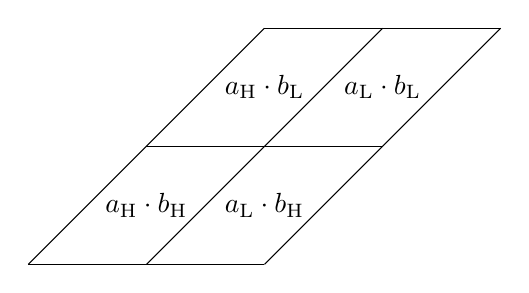
\begin{tikzpicture}[xslant = 1, scale = 1.5]
    \draw (0,0) -- (2,0);
    \draw (0,1) -- (2,1);
    \draw (0,2) -- (2,2);
    \draw (0,0) -- (0,2);
    \draw (1,0) -- (1,2);
    \draw (2,0) -- (2,2);
    \node at (.5,.5) {$a_\mathrm H\cdot b_\mathrm H$};
    \node at (1.5,.5) {$a_\mathrm L\cdot b_\mathrm H$};
    \node at (.5,1.5) {$a_\mathrm H\cdot b_\mathrm L$};
    \node at (1.5,1.5) {$a_\mathrm L\cdot b_\mathrm L$};
  \end{tikzpicture}
\caption{\llabel{fig:school}
  Illustration af den rekursive udgave af skolemetoden for multiplikation.
  Hele parallellogrammet repræsenterer de $n^2$ ciffervise delprodukter, som optræder ved multiplikationen af $a$ og $b$.
  De fire mindre parallellogrammer svarer til produkterne $a_\mathrm H\cdot b_\mathrm H$, 
  $a_\mathrm H \cdot b_\mathrm L$, $a_\mathrm L \cdot b_\mathrm H$ og $a_\mathrm L \cdot b_\mathrm L$.
  I den rekursive udgave beregnes først cifferprodukterne i de fire delområder og siden, i et separat skridt, de fire resulterende summer.}   
\end{figure}

Hvordan hænger den rekursive multiplikationsalgoritme og skolemetoden sammen?
Metoderne er nært beslægte i den forstand, at de begge beregner samtlige $n^2$ cifferprodukter $a_i\cdot b_j$, hvilket resulterer i $2n^2$ cifre, som (forskudt efter deres cifferposition) lægges sammen for at danne  produktet $a\cdot b$.
%TODO crap in original, also clashes with code
Forskellen mellem metoderne ligger i rækkefølgen, hvori disse summering foregår.
Figur~\lref{fig:school} viser skematisk cifferprodukterne og deres position som parallellogram.
I skolemetoden lægges cifferprodukterne samme linje for linje, mens den rekursive metode løser de fire delproblemer i hver af de fire dele, og lægges dem sammen i tre afsluttene additioner.
Denne betragtning gør det desuden åbenbart, at antallet af elemantaroperationer er kvadratisk også i den rekursive udgave.
Alligevel vil vi også udlede udførelsestiden direkte ud fra en analyse af den rekursive algoritme.
I den sammenhæng vil vi støde på en såkaldt \emph{rekursionsligning}, et slags udtryk, som ofte optræder ved analysen rekursive algoritmer.

\begin{lemma}\llabel{thm:recursive school help} 
  Lad $T(n)$ være det maskimal antal elementaroperationer, som skal bruges til den rekursive multiplikationsalgoritme for to $n$-cifrede tal. 
  Da gælder:
  \begin{equation*}
    T(n) \le 
    \begin{cases}
      1\,,   & \text{når $n = 1$}\,; \\
      4 \cdot T(\ceil{n/2}) + 2 \cdot 2 \cdot n\,, & \text{når $n \ge 2$}\,.
    \end{cases}
  \end{equation*}
\end{lemma}

\begin{proof} 
  Multiplikationen af to etcifrede tal kræver en elementaroperation.
  Dermed gælder påstanden for $n=1$. 
  Antag $n\ge 2$.
  Opdelingen af tallene $a$ og $b$ i de fire dele $a_\mathrm H$, $a_\mathrm L$, $b_\mathrm H$ kræver  $b_\mathrm L$ ingen elementaroperationer.
  \footnote{Selvfølgeligt kræver dette skridt beregningstid, men denne tages altså ikke hensyn til i analysen.}
  Hvert af de fire tal har højst $\ceil{n/2}$ cifre, så de fire rekursive multiplikationer bruger sammenlagt ikke mere end $4 \cdot T(\ceil{n/2})$ elementaroperationer.
  Sammenføjningen af
  $a_\mathrm L\cdot b_\mathrm L$ og $a_\mathrm H\cdot b_\mathrm H\cdot B^{2k}$ til et tal koster ingen elementaroperationer, idet $a_\mathrm L\cdot b_\mathrm L$ kun består af $2k$ cifre og $a_\mathrm H\cdot b_\mathrm H\cdot B^{2k}$ ender med $2k$ nuller.
  %TODO wtf k?
  Afslutningsvist bruges to additioner til at beregne det endelige resultat.
  Hver af disse additioner behandler to tal med højst $2n$ cifre og bruger derfor højst
  $2n$ elementaroperationer.
  Derfor gælder også uligheden for $n\ge2$.
\end{proof}

I afsnnit~\ref{ch:intro:s:analysis} skal vi se, hvordan man løser rekursionsligningen i lemma~\lref{thm:recursive school help} for at etablere den formodede kvadratiske udførelsestid for den rekursive algoritme.
\index{rekursionsligning}
\index{algoritmeanalyse!rekursion} 

\begin{lemma}\llabel{thm:recursive school} 
   Lad $T(n)$ være det maskimal antal elementaroperationer, som skal bruges til den rekursive multiplikationsalgoritme for to $n$-cifrede tal. 
  Da gælder $T(n) \le 5n^2$, når $n$ er en topotens, og $T(n) \le 20n^2$ for vilkårlige naturlige tal $n$.  
\end{lemma}
\begin{proof} Se afsnit~\lref{s:proofs}.
\end{proof}

%%%%%%%%%%%%%%%%%%%%%%%%%%%%%%%%%%%%%%%%%%%%%%%%%%%%%%%%%%%%%%%%%%%%%%
\section{Karatsubamultiplikation}%
\index{multiplikation (naturlige tal)!Karatsuba|textbf}%
\index{algoritmekonstruktion!rekursion}
\index{rekursionsligning}
\index{algoritmeanalyse!rekursiv} 

År 1962 opdagede denn sovjetiske matematiker A.~Karatsuba~\cite{Karatsuba}
\index{Karatsuba, A.}
\index{Ofman, Y.}
en hurtigere metode til multiplikation af store naturlige tal.
Hans algoritmes udførelsestid vokser omtrent som  $n^{\log 3} \approx n^{\num{1.585}}$.
Metoden er overraskende nem.
Karatsuba lagde mærke til, at man kan spare en af multiplikationerne i del-og-hersk-udgaven basered på en enkel lighed mellem to termer.
Det vil sige, at man kan gange to $n$-cifrede tal sammen ved at gange  blot \emph{tre} tal af den halve længde.

Vi vil nu beskrive denne tilgang i detaljer.
Lad $k=\floor{n/2}$. 
Som før kalder vi multiplikationens to operander for $a$ og $b$ og deler $a$ i to tal $a_\mathrm H$ og $a_\mathrm L$, hvor $a_\mathrm L$ er de $k$ lavestbetydende cifre i $a$ og 
$a_\mathrm H$ er de resterene $n - k$ højestbetydende cifre. 
På samme måde opdeles $b$ i $b_\mathrm L$ og $b_\mathrm H$.
Da gælder
\[ a = a_\mathrm H \cdot B^{k} + a_\mathrm L  \quad \text{og} \quad b = b_\mathrm H \cdot B^{k} + b_\mathrm L \,,\]
og derfor (trikket er i den anden ligning!)
\begin{multline*}
a\cdot b = a_\mathrm H\cdot b_\mathrm H\cdot B^{2k} + (a_\mathrm H\cdot b_\mathrm L + a_\mathrm L \cdot b_\mathrm H)\cdot B^k
+ a_\mathrm L\cdot b_\mathrm L = \\
          a_\mathrm H\cdot b_\mathrm H\cdot B^{2k} + ( (a_\mathrm H + a_\mathrm L)\cdot(b_\mathrm H + b_\mathrm L) -
(a_\mathrm H\cdot b_\mathrm H + a_\mathrm L \cdot b_\mathrm L))\cdot B^k
+ a_\mathrm L\cdot b_\mathrm L \,.
\end{multline*}
Umiddelbart ser det jo ud, som om vi bare har gjort tingene mere komplicerede.
Men ved nærmere syn ser man, at det sidste udtryk kun bruger tre multiplikationer af kortere tal, nemlig beregningen af $a_\mathrm H\cdot b_\mathrm H$, $a_\mathrm L \cdot b_\mathrm L$ og $(a_\mathrm H + a_\mathrm L) \cdot (b_\mathrm H + b_\mathrm L)$.
Der kræves også fem additioner,
\footnote{For at være nøjagtig, skal man bruge fire additioner og en subtraktion.
Vi overlader det til læseren at overbevise sig om, at subtraktion ikke er dyrere end addition.
}
hvilket er tre mere end i den rekursive udgave af skolemetoden.
Men det afgørende er, at additionerne (som udføres umiddelbart)  er meget billige i forhold til multiplikationerrne (som er rekursive), hvorfor det er giver mening at spare en multiplikation for prisen af tre additioner.
Vi har altså følgende  algoritme for at beregne $a \cdot b$:

\begin{enumerate}[(a)]
\item Opdel $a$ og $b$ i $a_\mathrm H$, $a_\mathrm L$, $b_\mathrm H$ og $b_\mathrm L$.
\item Beregn de tre produkter 
\[ p_2 = a_\mathrm H\cdot b_\mathrm H,\quad p_0 = a_\mathrm L  \cdot b_\mathrm L, \quad
p_1 = (a_\mathrm H + a_\mathrm L) \cdot (b_\mathrm H + b_\mathrm L).\]
\item Læg produkterne fra (b) sammen, passende forskudte, for at danne produktet $a \cdot b$, dvs. som
\[ a\cdot b = (p_2 \cdot B^{2k} + p_0) + ( p_1 - (p_2 + p_0))\cdot B^k\,.\]
(Den første sum er bare en sammenføjning af to tal, ikke en rigtig addition.)
\end{enumerate}

Tallene $a_\mathrm H$, $a_\mathrm L$, $b_\mathrm H$, $b_\mathrm L$, $a_\mathrm H + a_\mathrm L$ og $b_\mathrm H + b_\mathrm L$ består af højst $\ceil{n/2} + 1$ cifre. 
Derfor er multiplikationen i skridt~(b) enklere end den oprindelige opgave, såfremt $\ceil{n/2} + 1 < n$, dvs. $n \ge 4$.
Den fuldstændige algoritme kan nu beskrives på følgende måde:
For at multiplicere tal med tre cifre eller mindre, benytter man skolemetoden.
For tal med $n\ge4$ cifre bruges tretrinsmetoden foroven.

\begin{figure}[h]  %\begin{wrapfigure}{o}{0.6\textwidth} does not work
\sidecaption
  \begin{minipage}{0.5\textwidth}
    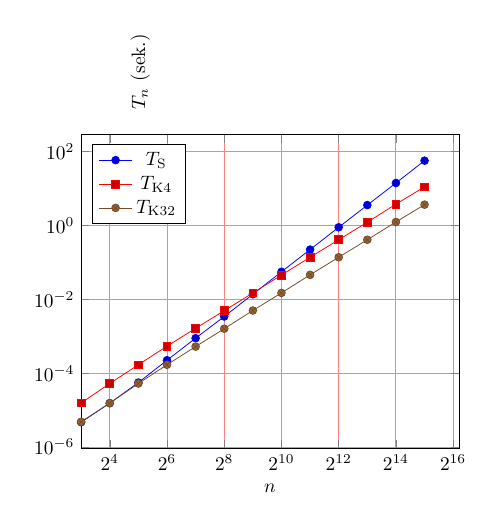
\begin{tikzpicture}[scale = .7]
    \begin{loglogaxis} [xlabel=$n$, xmin = 8, ylabel=$T_n$ (sek.),   log basis x={2},     grid=both,
      y label style = { at = {(0.2,1.2)}, anchor = south},
      major grid style={red!50}, legend pos = {north west}]
\addplot table[x=n,y = school, row sep=crcr] {
n      school      LEDAtime    Karatsuba4  Karatsuba32\\
8      4.72378e-06 4.48759e-06 1.56597e-05 4.84041e-06\\
16     1.54231e-05 1.51177e-05 5.26565e-05 1.55214e-05\\
32     5.58285e-05 5.19205e-05 0.000169233 5.25956e-05\\
64     0.000224417 0.000222172 0.000539374 0.000169205\\
128    0.000888099 0.000870338 0.00164228  0.00052521\\
256    0.00342373  0.00342373  0.00492611  0.00160256\\
512    0.0136986   0.0136986   0.0148529   0.00497512\\
1024   0.0555556   0.055       0.0454545   0.0149254\\
2048   0.222       0.222       0.1375      0.0459091\\
4096   0.89        0.885       0.41        0.1375\\
8192   3.55        3.54        1.22        0.41\\
16384  14.07       14.07       3.76        1.24\\
32768  56.6        56.48       11.09       3.65\\
  	};
\addplot table[x=n,y = Karatsuba4, row sep=crcr] {
n       Karatsuba4  Karatsuba32\\
8       1.56597e-05 4.84041e-06\\
16      5.26565e-05 1.55214e-05\\
32      0.000169233 5.25956e-05\\
64      0.000539374 0.000169205\\
128     0.00164228  0.00052521\\
256     0.00492611  0.00160256\\
512     0.0148529   0.00497512\\
1024    0.0454545   0.0149254\\
2048    0.1375      0.0459091\\
4096    0.41        0.1375\\
8192    1.22        0.41\\
16384   3.76        1.24\\
32768   11.09       3.65\\
  	};
\addplot table[x=n, row sep=crcr] {
n        Karatsuba32\\
8        4.84041e-06\\
16       1.55214e-05\\
32       5.25956e-05\\
64       0.000169205\\
128      0.00052521\\
256      0.00160256\\
512      0.00497512\\
1024     0.0149254\\
2048     0.0459091\\
4096     0.1375\\
8192     0.41\\
16384    1.24\\
32768    3.65\\
  	};
	\legend{$T_\mathrm S$,$T_{\mathrm K4}$,$T_{\mathrm K32}$}
	\end{loglogaxis}
\end{tikzpicture}
\end{minipage}
\caption{
  Eksperimentel sammenligning af udførelsestiden for to implementationer af Karatsubas algoritme og skolemetoden for multiplikation af naturlige tal. 
  Implementationen K4 skifter til skolemetoden for tal bestående af færre end fire cifre, K32 for tal med færre end 32 cifre. 
  Hældningen for de tilsvarende linjer er omtrent $\num{1.58}$. 
  K32 er tre gange hurtigere end K4.
\llabel{fig:comparison school Karatsuba}}
\end{figure}

\index{Algorithm Engineering}%
Figur~\lref{fig:comparison school Karatsuba} viser udførelsestiderne 
$T_S(n)$, $T_{K4}(n)$ og  $T_{K32}(n)$ for implementationer i \CC\ af skolemetoden og Karatsubas algoritme for multiplikation af $n$-cifrede tal.
Varianten K4 (med udførelsestid $T_{K4}(n)$) skifter til skolemetoden ved færre end fire cifre.
Forbedringen i varianten K32 (med udførelsestid $T_{K32}(n)$) beskrives i
afsnit~\lref{s:engineering}.
Begge akser bruger en logaritmisk skala.
Groft sagt viser figuren tre linjer med forskellig hældning.
Udførelsestiden $T_\mathrm S$ for skolemetoden vokser som~$n^2$, derfor har denn tilsvarende linje hældning ~$2$.
Linjen for  Karatsubas algoritme $T_{\mathrm K4}$ har en svagere hældning, hvilket tyder på, at udførelsestiden vokser som $n^\beta$ for en konstant $\beta < 2$.
Kvotienterne \footnote{$T_{K4}(1024) = \num{0.0455}$,
$T_{K4}(2048) = \num{0.1375}$ og $T_{K4}(4096) = \num{0.41}$.} 
$T_{K4}(n)/T_{K4}(n/2)$ 
og $T_{K32}(n)/T_{K32}(n/2)$ ligger tæt på~$3$, hvilket antyder, at $\beta$  opfylder ligningen $2^\beta = 3$, dvs. at der gælder $\beta = \log 3 \approx \num{1.585}$.    
Omtrent samme hælding kan også aflæses af figur~\lref{fig:comparison school Karatsuba}, og forneden beviser vi formelt, at $T_{K4}(n)$ vokser som  
$n^{\log 3}$.
For at sammenfatte disse betragtninger siger vi, at Karatsubas algoritme er \emph{asymptotisk hurtigere} 
\index{asymptotisch}
end skolemetoden.
Men vi indser også, at instanserne skal være meget store, inden karatsubaalgoritmens bedre asymptotiske opførsel gør sig gældende i form af et faktisk mindsket tidsforbrug.
Læg mærke til, at skolemetoden stadig her hurtigere end K4 for $n=2^8$, at algoritmerne er lige hurtige for $n=2^9$, og at Karatsubas algoritme vinder fra og med $n=2^{10}$.
Disse betragtninger fortæller os, at
\begin{itemize}
\item bedre asymptotisk opførsel vinder i sidste ende,
%However, it may lose on small inputs. 
\item en asymptotisk langsommere algoritme kan være hurtigere på små instanser.
%You may only be interested in small inputs.
\end{itemize}
I næste afsnit skal vi se, hvordan man kan forbedre Karatsubas algoritme for små $n$ og derved opnå en algoritme, som er mindst lige så god som skolemetoden. 

Nu kommer vi  endelig til den grundige analyse af Karatsubas algoritme.

\begin{lemma}\llabel{lem:karatsuba help} 
  Lad $T_K(n)$ være det maksimale antal elementaroperationer, som Karatsubas algortime bruger på $n$-cifrede tal.
  Da gælder:
\begin{equation*}
T_K(n) \le 
\begin{cases}
3n^2  & \text{når $n \le 3$}, \\
3 \cdot T_K(\ceil{n/2} + 1) + 8 n  & \text{når $n \ge 4$}.
\end{cases}
\end{equation*}
\end{lemma}
\begin{proof} 
  For $n\le3$ bruger vi sætning~\lref{thm:eff of school method}, som siger, at multiplikationen af to $n$-cifrede tal med skolemetoden bruger højst $3n^2$ elementaroperationer.
  Betragt nu tilfældet $n\ge4$. 
  Opdelingen af $a$ og $b$ i fire dele $a_\mathrm H$, $a_\mathrm L$, $b_\mathrm H$ und $b_\mathrm L$ bruger ingen elementaroperationer (jf. fodnoten i beviset for lemma~~\lref{thm:recursive school help}).
  Alle dele samt summerne $a_\mathrm L + a_\mathrm H$ og $b_\mathrm L + b_\mathrm H$ har hver højst $\ceil{n/2} + 1 $ cifre; så det tre rekursive multiplikationer bruger højst $3 \cdot T_K(\ceil{n/2} + 1)$ elementaroperationer. 
  For at danne summerne $a_\mathrm L + a_\mathrm H$ og $b_\mathrm L + b_\mathrm H$ skal vi bruge to additioner, hvis resultatet hver har færre end $n$ cifre, så vi bruger $2n$ elementaroperationer. 
  Endelig bruges tre additioner af højst $2n$-cifrede tal for at udregne resultatet fra de tre produkter, hvilket kræver højst $3\cdot 2n$ yderligere elementaroperationerer.
  Sammenlagt giver dette den øvre grænse i lemmaet for $n\ge4$.
\end{proof} 

I afsnit~\ref{ch:intro:s:analysis} viser vi, hvordan man kan løse rekursionsligninger af denne type generelt.

\begin{thm}
  \llabel{thm:Karatsuba}
  Lad $T_K(n)$ være det maksimale antal elementaroperationer, som Karatsubas algortime bruger til multiplikation af to $n$-cifrede tal.
  Da gælder $T_K(n) \le 153 n^{\log 3}$ for alle $n$. 
\end{thm}
\begin{proof} 
  Se afsnit~\lref{s:proofs}. 
\end{proof}


%%%%%%%%%%%%%%%%%%%%%%%%%%%%%%%%%%%%%%%%%%%%%%%%%%%%%%%%%%%%%%%%%%%%%%
\section{Algoritmeoptimering}
\index{Algorithm Engineering}
\llabel{s:engineering}

\emph{Udeladt}

%(\begin{comment}
%(Die Karatsuba-Methode für die Multiplikation von 
%(natürlichen Zahlen ist für große Eingaben besser als die Schulmethode.
%(In unserer Implementierung Karatsuba4 zeigt sich die Überlegenheit
%(erst für Zahlen mit mehr als 1000 Ziffern. 
%(Durch eine sehr einfache Verfeinerung 
%(lässt sich das Rechenzeitverhalten aber deutlich verbessern.
%(Weil für kurze Zahlen die Schulmethode besser ist, 
%(sollten wir die Rekursion schon früher
%(abbrechen und für Zahlen mit
%($n_0$ und weniger Ziffern auf die Schulmethode umschalten,
%(für ein $n_0$, das wir passend bestimmen müssen. 
%(Diesen Ansatz nennen wir die \index{Multiplikation (natürlicher Zahlen)!Karatsuba!verfeinert}\emph{verfeinerte Karatsuba-Methode}.
%(Er kann nie schlechter sein als die Schulmethode 
%(oder der einfache Karatsuba-Algorithmus, solange $n_0$ nicht zu groß ist.  
%(
%(\begin{figure}%{o}{0.5\textwidth}
%(\sidecaption
%({\begin{sideways}\parbox{5cm}{\centerline{\sf time [sec]}}\end{sideways}}%
%(\includegraphics[width=0.5\textwidth]{\masterdir/amuse/Experiments/abhaengigkeit.eps}
%(\caption{Die Rechenzeit des Karatsuba-Algorithmus (in Sekunden) in Abhängigkeit von 
%(der Rekursionsschwelle $n_0$.
%(Dargestellt sind die Zeiten für die Multiplikation von Zahlen mit $2048$ Ziffern
%(bzw. Zahlen mit $4096$ Ziffern. Das Minimum ist bei $n_0 = 32$.}
%(\llabel{fig: refined Karatsuba}
%(\end{figure}
%(Was ist ein guter Wert für~$n_0$?
%(Diese Frage wollen wir sowohl mit Hilfe eines
%(Experiments als auch durch eine Analyse beantworten. 
%(Experimentell messen wir einfach die Rechenzeit,
%(die der verfeinerte Karatsuba-Algorithmus für 
%(verschiedene Schwellwerte $n_0$ benötigt,
%(und wählen den Wert, der die kleinste Rechenzeit liefert. 
%(Für unsere Implementierung ergaben sich die besten 
%(Ergebnisse für $n_0 = 32$ (s. Abb.~\lref{fig: refined
%(Karatsuba}). 
%(Das asymptotische Verhalten des verfeinerten Karatsuba-Algorithmus
%(mit diesem Schwellwert ist
%(Abb.~\lref{fig:comparison school Karatsuba} dargestellt.
%(Wir sehen, dass die Rechenzeit ebenfalls wie $n^{\log 3}$ wächst.
%(Die verfeinerte Methode ist aber etwa um den Faktor 3 schneller
%(als der einfache Karatsuba-Algorithmus, ist also eine
%(sehr wirkungsvolle Verbesserung, und sie ist niemals 
%(langsamer als die Schulmethode.      
%(
%(\begin{exerc}\llabel{ex:refined Karatsuba} 
%(Leiten Sie eine Rekurrenz für die Anzahl $T_R(n)$ 
%(von Elementaroperationen her, die beim verfeinerten Karatsuba-Algorithmus
%(im schlechtesten Fall auftreten können. 
%(\end{exerc}
%(
%(\index{Algorithmenanalyse!rekursiv}%
%(Wir können die Frage auch analytisch angehen. 
%(Die Schulmethode benötigt nicht mehr als $3n^2$ Elementaroperationen
%(für die Multiplikation von zwei $n$-ziffrigen Zahlen. 
%(Wenn wir einen Karatsuba-Schritt ausführen und die 
%(resultierenden Zahlen der Länge $\ceil{n/2} + 1$ mit der Schulmethode
%(multiplizieren, benötigen wir etwa $3 \cdot 3(n/2 + 1)^2 + 8n$ Elementaroperationen.
%(Der letzte Ausdruck ist für $n\ge24$ kleiner als $3n^2$,
%(und daher spart ein rekursiver Schritt Elementaroperationen ein, 
%(sobald die Eingabezahlen mehr als 24 Ziffern haben. 
%(Nun sollte man diese Überlegung nicht einfach zum Anlass nehmen, 
%(die Schwelle für die Rekursion bei etwa 24 Ziffern anzusetzen.
%(Sie beruht ja nur auf Schätzwerten und berücksichtigt nur die Elementaroperationen.
%(Vielmehr sollte man aus unserer Überlegung schließen, 
%(dass es sinnvoll ist, eine nichttriviale Rekursionsschwelle $n_0$ zu benutzen,
%(und ein geeignetes $n_0$ experimentell bestimmen. 
%(
%(\begin{exerc}\llabel{ex:karatsuba:subtract}
%(Entwickeln und analysieren Sie eine Variante der Karatsuba-Multi\-pli\-ka\-tion,
%(die das Entstehen von Übertragsziffern bei der Summenbildung $a_\mathrm H+a_\mathrm L$ bzw. $b_\mathrm H+b_\mathrm L$ vermeidet. 
%(\emph{Hinweis}:
%(Bilden Sie $p_0$ und $p_2$ wie vorher, setzen Sie jedoch $p_1'=(a_\mathrm H-a_\mathrm L)\cdot(b_\mathrm H-b_\mathrm L)$
%(und verändern Sie die Formel zur Ermittlung des Ergebnisses $a\cdot b$ in passender Weise. 
%(Was kann man über die Anzahl der Ziffern der Absolutbeträge $|a_\mathrm H-a_\mathrm L|$ und $|b_\mathrm H-b_\mathrm L|$ sagen,
%(wenn $a$ und $b$ jeweils $n$ Ziffern haben?
%(Nehmen Sie an, dass ganze Zahlen als Kombination von Vorzeichen und Absolutbetrag 
%(dargestellt sind, und schätzen Sie die Anzahl der für Größenvergleiche, Additionen und Subtraktionen 
%(nötigen Elementaroperationen ab. 
%(Passen Sie die Rekurrenz für die
%(Elementaroperationen aus Lemma~\lref{lem:karatsuba help} an die veränderte Situation an.
%(Lösen Sie die Rekurrenz für den Fall, dass $n$ eine Zweierpotenz ist. 
%(\end{exerc}
%(
%(\begin{exerc} 
%(In diesem Kapitel haben wir stets angenommen, dass die beiden zu 
%(multiplizierenden Zahlen gleich viele Ziffern haben. 
%(Was kann man über den Aufwand für die Multiplikation 
%(einer $n$-ziffrigen Zahl $a$ mit einer $m$-ziffrigen Zahl $b$ sagen?
%((a) Zeigen Sie, dass die Schulmethode nicht mehr als
%($\alpha \cdot nm$ Elementaroperationen benötigt, für eine Konstante $\alpha$.
%((b) Wenn $n\ge m$ ist, können wir $a$ in $\ceil{n/m}$ Zahlen mit je $m$ Ziffern
%(einteilen und mit dem Karatsuba-Algorithmus jedes der Teilstücke mit $b$
%(multiplizieren. Dann sind noch die Teilergebnisse zu kombinieren.
%(Bestimmen Sie eine Schranke für die Anzahl der Elementaroperationen bei diesem Ansatz.
%(\end{exerc}
%(
%(\end{comment}

%%%%%%%%%%%%%%%%%%%%%%%%%%%%%%%%%%%%%%%%%%%%%%%%%%%%%%%%%%%%%%%%%%%%%%%%%%%%%%%%%%%%%%%%%%%%%%%%%%%%%%%%%%%%%%%%
\section{Programmerne}
\llabel{s: programs}
%%%%%%%%%%%%%%%%%%%%%%%%%%%%%%%%%%%%%%%%%%%%%%%%%%%%%%%%%%%%%%%%%%%%%%%%%%%%%%%%%%%%%%%%%%%%%%%%%%%%%%%%%%%%%%%%

\emph{Udeladt}
%\begin{comment}
%In diesem Abschnitt geben wir \CC-Programme für die Schulmethode und für die 
%beiden Varianten des Karatsuba-Algorithmus an. 
%Diese Programme wurden auch für die Rechenzeit-Experimente dieses Kapitels benutzt.
%Dafür wurden sie auf einem Rechner mit einem Intel-T7200-Prozessor (2\,GHz, Dual-Core)
%mit 4\,Mbyte Cache\-speicher und 2\,Gbyte Hauptspeicher ausgeführt.
%Übersetzt wurden die Programme mit dem
%GNU \CC-Compiler Version 3.3.5, Optimierungslevel \verb|-O2|.
%
%\newcommand{\mytt}[1]{{\renewcommand\ttdefault{cmss}\small\texttt{#1}}}
%
%Eine Ziffer (Typ "`\Id{digit}"') ist einfach ein \Id{unsigned\;int},
%und eine natürliche Zahl (Typ "`\Id{integer}"') ist ein Vektor von Ziffern,
%wobei "`Vektor"' der Vektortyp der STL\index{STL} ist.
%Eine Deklaration \Id{integer\ a(n)} deklariert eine natürliche Zahl mit $n$ Ziffern,
%\Id{a.size()} liefert die Länge von \Id{a} und \Id{a[i]} liefert einen
%Zeiger auf die $i$-te Ziffer von \Id{a}.     
%Die Nummerierung der Ziffern beginnt bei 0.
%Die globale Variable $B$ enthält die Basis. 
%Die Funktionen \Id{fullAdder} und \Id{digitMult}
%implementieren die Elementaroperationen auf den Ziffern. 
%Mitunter sollen Indizes $i$ benutzt werden, die 
%außerhalb des durch die Größe von \Id{a} gegebenen Bereichs liegen.
%Hierfür benutzen wir die Funktion \Id{getDigit(a,i)},
%die \Id{a[i]} liefert, wenn \Id{i} ein für \Id{a} legaler
%Index ist, und $0$ sonst.       
%
%Wir wollen unsere Programme auf zufälligen Zahlen ablaufen lassen: \Id{randDigit} 
%ist ein einfacher (Pseudo-)Zufallszahlengenerator für Ziffern, und \Id{randInteger} 
%erzeugt damit zufällige Ziffern, um mit diesen sein Argument zu füllen.
%
%{\small
%\begin{verbatim}
%   unsigned int X = 542351;
%   digit randDigit() { X = 443143*X + 6412431; return X % B ; }
%   void randInteger(integer& a)
%   { int n = a.size(); for (int i=0; i<n; i++) a[i] = randDigit(); }
%\end{verbatim}
%}
%
%Wir kommen nun zur Schulmethode. Zunächst beschreiben wir ein Unterprogramm \Id{mult},
%das eine Zahl \Id{a} mit einer Ziffer \Id{b} multipliziert und das Ergebnis
%als Zahl \Id{atimesb} zurückgibt. 
%Es wird eine Übertragsziffer \Id{carry} benötigt, die mit $0$ initialisiert wird.  
%Im Schleifendurchlauf für $i$ berechnen wir zunächst Ziffern $d$ und $c$ mit $c\cdot B + d = a[i]\cdot b$.   
%Die Summe von $d$ und dem Wert $c$ und den Übertrag \Id{carry}
%aus dem vorherigen Schleifendurchlauf ergibt eine Summenziffer,
%die in $\Id{atimesb}[i]$ gespeichert wird, und einen neuen Übertrag \Id{carry}.
%Die Schulmethode (die Funktion \Id{mult}) multipliziert \Id{a} mit jeder Ziffer von \Id{b}
%und addiert (mittels der Funktion \Id{addAt}) dieses Teilprodukt, 
%um die korrekte Anzahl von Stellen verschoben, zum bisher aufgelaufenen Ergebnis.    
%
%{\small
%\begin{verbatim}
%   void mult(const integer& a, const digit& b, integer& atimesb)
%   { int n = a.size(); assert(atimesb.size() == n+1);
%     digit carry = 0, c, d, cprev = 0;
%     for (int i = 0; i < n; i++) 
%       { digitMult(a[i],b,d,c); 
%	 fullAdder(d, cprev, carry, atimesb[i], carry); cprev = c; 
%       }
%     d = 0;
%     fullAdder(d, cprev, carry, atimesb[n], carry);  assert(carry == 0);
%   }
%   void addAt(integer& p, const integer& atimesbj, int j)
%   { // p hat Laenge n+m, 
%     digit carry = 0; int L = p.size();
%     for (int i = j; i < L; i++) 
%       fullAdder(p[i], getDigit(atimesbj,i-j), carry, p[i], carry);
%     assert(carry == 0);
%   }
%   integer mult(const integer& a, const integer& b)
%   { int n = a.size(); int m = b.size();
%     integer p(n + m,0);  integer atimesbj(n+1);
%     for (int j = 0; j < m; j++) 
%       { mult(a, b[j], atimesbj); addAt(p, atimesbj, j); }
%     return p;
%   }
%\end{verbatim}
%}
%
%
%Für die Implementierung des Karatsuba-Algorithmus benötigen wir auch
%Programme für die allgemeine Addition und die Subtraktion.
%Bei der Subtraktion kann angenommen werden, dass
%das zweite Argument nicht größer als das erste ist.
%Die Differenz wird dann im ersten Argument zurückgegeben. 
%
%{\small
%\begin{verbatim}
%   integer add(const integer& a, const integer& b)
%   { int n = max(a.size(),b.size());
%     integer s(n+1); digit carry = 0; 
%     for (int i = 0; i < n; i++) 
%	 fullAdder(getDigit(a,i), getDigit(b,i), carry, s[i], carry); 
%     s[n] = carry;
%     return s;
%   }
%   void sub(integer& a, const integer& b) // setzt a >= b voraus
%   { digit carry = 0; 
%     for (int i = 0; i < a.size(); i++) 
%       if ( a[i] >= ( getDigit(b,i) + carry )) 
%	  { a[i] = a[i] - getDigit(b,i) - carry; carry = 0; }
%       else { a[i] = a[i] + B - getDigit(b,i) - carry; carry = 1; }
%     assert(carry == 0);
%   }
%\end{verbatim}
%}
%
%Die Funktion \Id{split} zerlegt eine Zahl in zwei Zahlen der halben Länge:
%
%{\small
%\begin{verbatim}
%   void split(const integer& a,integer& a1,  integer& a0)
%   { int n = a.size(); int k = n/2;
%     for (int i = 0; i < k; i++) a0[i] = a[i];
%     for (int i = 0; i < n - k; i++) a1[i] = a[k + i];
%   }
%\end{verbatim}
%}
%
%Die Funktion \Id{Karatsuba} geht genauso vor wie im Text beschrieben. 
%Wenn die Eingabezahlen weniger als \Id{n0} Ziffern haben,
%wird die Schulmethode benutzt. 
%Andernfalls werden die Eingabezahlen in je zwei Teile der halben Länge zerlegt
%und die Produkte \Id{p0}, \Id{p1} und \Id{p2} werden gebildet. 
%Anschließend werden \Id{p0} und \Id{p2} einerseits an die korrekte Position in den Ausgabevektor geschrieben
%und andererseits nacheinander von \Id{p1} subtrahiert. 
%Die so modifizierte Zahl \Id{p1} wird, 
%um die korrekte Anzahl von Stellen verschoben, 
%zum bisherigen Ergebnis addiert. Dies liefert folgendes Programm: 
%
%{\small
%\begin{verbatim}
%   integer Karatsuba(const integer& a, const integer& b, int n0)
%   { int n = a.size(); int m = b.size(); assert(n == m); assert(n0 >= 4); 
%     integer p(2*n);
%
%     if (n < n0) return mult(a,b);
%
%     int k = n/2; integer a0(k), a1(n - k), b0(k), b1(n - k); 
%
%     split(a,a1,a0); split(b,b1,b0);
%
%     integer p2 = Karatsuba(a1,b1,n0), 
%	     p1 = Karatsuba(add(a1,a0),add(b1,b0),n0), 
%	     p0 = Karatsuba(a0,b0,n0);  
%
%     for (int i = 0; i < 2*k; i++) p[i] = p0[i];        
%     for (int i = 2*k; i < n+m; i++) p[i] = p2[i - 2*k];   
%
%     sub(p1,p0); sub(p1,p2); addAt(p,p1,k);
%
%     return p;
%   }
%\end{verbatim}
%}
%Die Daten für Abb.~\lref{fig:comparison school Karatsuba} 
%wurden von folgendem Programm erzeugt:
%
%{\small
%\begin{verbatim}
%   inline double cpuTime() { return double(clock())/CLOCKS_PER_SEC; }
%
%   int main(){ 
%
%   for (int n = 8; n <= 131072; n *= 2) 
%   { integer a(n),  b(n); randInteger(a); randInteger(b);
%
%     double T = cpuTime();  int k = 0;
%     while (cpuTime() - T < 1) {  mult(a,b); k++; }
%     cout << "\n" << n << " school = " << (cpuTime() - T)/k;
%
%     T = cpuTime(); k = 0;
%     while (cpuTime() - T < 1) {  Karatsuba(a,b,4); k++; }
%     cout << " Karatsuba4 = " << (cpuTime() - T) /k; cout.flush(); 
%
%     T = cpuTime(); k = 0;
%     while (cpuTime() - T < 1) {  Karatsuba(a,b,32); k++; }
%     cout << " Karatsuba32 = " << (cpuTime() - T) /k; cout.flush();   
%   }
%   return 0;
%   }
%\end{verbatim}
%}
%
%\end{comment}

\section{Bevis for lemma~\lref{thm:recursive school} og sætning~\lref{thm:Karatsuba}}
\llabel{s:proofs}


\index{algoritmenanalyse!rekursion}
\index{rekursionsligning}
For fuldstændighedens skyld beviser vi lemma~\lref{thm:recursive school} og sætning~\lref{thm:Karatsuba}.
Vi begynder med analysen af den rekursive udgave af skolemetoden.
I lemma~\lref{thm:recursive school help} har vi set, at det maksimale antal elementaroperationer, som skal bruges til multiplkation af to $n$-cifrede tal, opfylder rekursionsligningen
\begin{equation*}
T(n) \le 
\begin{cases}
1\,,   & \text{når $n = 1$}\,; \\
4 \cdot T(\ceil{n/2}) + 4n \,, & \text{når $n \ge 2$}\,.
\end{cases}
\end{equation*}
Ved induktion i $n$ viser vi, at $T(n) \le 5n^2 - 4n$, når $n$ er en topotens. 
For $n = 1$ har vi $T(1) \le 1 = 5n^2 - 4n$. 
For topotens $n$ med $n > 1$ gælder
\[ T(n) \le 4\cdot T(n/2) + 4n \le 4 (5 (n/2)^2 - 4n/2) + 4 n = 5n^2 - 4n \,;
\]
hvor den anden ulighed gælder ved induktion.
For vilkårlig $n$ observerer vi, at multiplkationsalgoritmen på to $n$-cifrede tal ikke kan være dyrere end på to $2^{\lceil\log n\rceil}$-cifrede tal, idet $n =2^{\log n} \leq 2^{\lceil\log n\rceil}$.
Derfor gælder $T(n) \le T(2^{\ceil{\log n}})$.
Idet $2^{\ceil{\log n}}\leq 2^{1+\log n} = 2n$, får vi den øvre grænse $T(n) \le 20 n^2$ for alle $n$.    

\begin{exerc} 
  Givet rekursionsligningen $T(1) \le 1$ und $T(n) \le 4 \cdot T(n/2) + 9n$.
  Vis en øvre grænse på $T(n)$ når  $n$ er en topotens.
\end{exerc}

Hvordan kunne vi vide i forvejen, at »$5n^2 - 4n$«  var den grænse, som fik induktionsbeviset til at holde?
Det kræver ikke, at man er synsk.
For $n = 2^k$ får vi ved gentagen substitution:
\begin{align*}
T(2^k) &\le 4 \cdot T(2^{k-1}) + 4\cdot2^k 
       \le 4^2 \cdot T(2^{k-2}) + 4 \cdot ( 4^1 \cdot 2^{k-1} + 2^k)\\
       &\le  4^3 \cdot T(2^{k-3}) + 4 \cdot ( 4^2 \cdot 2^{k-2} + 4^1 \cdot 2^{k-1} + 2^k
) \le \cdots\\
&\le 4^k\cdot T(1) + 4 \cdot \sum_{0 \le i \le k-1}\!\!4^i 2^{k-i} \le 4^k + 4
\cdot 2^k\cdot \sum_{0 \le i \le k-1}\!\!2^i\\
&\le 4^k + 4 \cdot 2^k (2^k - 1)
= n^2 + 4n(n - 1) = 5n^2 - 4n\,.
\end{align*}

Nu til beviset for sætning~\lref{thm:Karatsuba}.
Fra lemma~\lref{lem:karatsuba help} ved vi, at $T_K$ opfylder følgende rekursionsligning:
\begin{equation*}
T_K(n) \le 
\begin{cases}
3n^2\,, & \text{når $n \le 3$}\,; \\
3 \cdot T_K(\ceil{n/2} + 1) + 8 n \,,& \text{når $n \ge 4$}\,.
\end{cases}
\end{equation*}
Rekursionsligningen for skolemetoden havde den behagelige egenskab, at hvis $n$ var en topotens, så var argumenterne på højresiden af udtrykket også topotenser.
Det gælder ikke for $T_K$.
Men når $n$ er på formen $n = 2^k + 2$ og  $k \ge 1$, så gælder $\ceil{n/2} + 1
= 2^{k-1} + 2$. 
Vores induktionsbevis bør altså føres for tal på formen $n = 2^k + 2$ med $k\ge 0$.
Vi vil vise, at der for $k \ge 0$ gælder
\[   T_K(2^k + 2) \le 51\cdot 3^k - 16\cdot 2^k - 8\,. \]
For $k = 0$ har vi
\[ T_K(2^0 + 2) = T_K(3) \le 3\cdot 3^2  = 27 = 51\cdot 3^0 - 16\cdot 2^0 - 8 \,. \]
I induktionsskridtet for $k \ge 1$ gælder
\begin{align*}
  T_K(2^k + 2) &\le 3 \cdot T_K (2^{k-1} + 2) + 8 \cdot (2^k + 2)\\
  &\le 3\cdot \left(51\cdot 3^{k-1}  - 16\cdot 2^{k-1} - 8\right) + 8 \cdot (2^k + 2)\\
  &= 51\cdot 3^k  - 16\cdot 2^k - 8\,. 
\end{align*}
Igen fandt vi den givtige induktionsantagelse uden heksekunster, med ved gentagen substitution:
\begin{align*}
T_K(2^k + 2) &\le 3 \cdot T_K(2^{k-1} + 2) + 8\cdot(2^k + 2)\\
             &\le 3^k \cdot T_K(2^0 + 2) + 8\cdot (3^0\cdot(2^k+2) + 3^1\cdot(2^{k-2}+2) + \ldots +
3^{k-1}\cdot(2^1+2))\\
             &\le 27\cdot 3^k + 8\cdot \left(2^k\cdot\frac{(3/2)^k-1}{3/2-1} + 2\cdot\frac{3^k-1}{3-1}\right) \\
             & = 51\cdot 3^k -16\cdot 2^k -8\,. 
\end{align*}
Endelig skal vi generalisere udtrykket til alle $n$.
Hertil vælger vi det mindste $k$, som opfylder $n\le 2^k+2$.
Åbenbart gælder $k \le 1 + \log n$. 
Multiplikationen af $n$-cifrede tal  kan ikke være dyrere end for tal med $2^k+2$ cifre. 
Heraf følger:
\begin{align*}
T_K(n) \le 51\cdot3^k - 16 \cdot 2^k - 8  \le 153\cdot3^{\log n} \le 153\cdot n^{\log 3}\,,
\end{align*}
hvor vi har brugt $3^{\log n} = 2^{(\log 3) \cdot (\log n)} = n^{\log 3}$.

\section{Implementationsaspekter}

\emph{Udeladt}
%Die in Abschnitt~\lref{s: programs} angegebenen Programme sind nicht optimiert. 
%Zum Beispiel sollte die Basis $B$ des benutzten Zahlensystems eine Zweierpotenz sein, 
%so dass man die Summen- und Übertragsziffern bei den Elementaroperationen
%durch einfache Bit\-opera\-tio\-nen aus den Ergebnissen der Maschinenoperationen erhält. 
%Auch sollte die Größe einer Ziffer der Wortlänge des Rechners entsprechen,
%und man sollte sich bei der Implementierung der Elementaroperationen mehr Mühe geben.
%
%\subsection{\protect\CC}\index{C++@\CC} 
%In den Paketen GMP~\cite{GMP}\index{GMP} und LEDA~\cite{LEDA-AS}\index{LEDA} 
%werden Langzahlarithmetik für ganze Zahlen, exakte Arithmetik für rationale Zahlen
%und beliebig genaue Arithmetik für Gleitkommazahlen\index{Gleitkommadarstellung} bereitgestellt. 
%Für die Multiplikation werden dabei stark optimierte Implementierungen 
%der Methode von Karatsuba benutzt. 
%
%\subsection{Java}\index{Java} Im Paket \Id{java}.\Id{math} werden beliebig lange 
%ganze Zahlen und beliebig genaue Gleitkommazahlen\index{Gleitkommadarstellung} bereitgestellt.
%

%%%%%%%%%%%%%%%%%%%%%%%%%%%%%%%%%%%%%%%%%%%%%%%%%%%%%%%%%%%%%%%%%%%%%%
\section{Historiske anmærkninger og yderligere resultater}
\llabel{s:further}

Er Karatsubas algoritme den hurtigst kendte multiplkationsalgoritme?
Nej, man kender meget hurtigere metoder.
Karatsubas algoritme deler $n$-cifrede tal op i to dele og klarer sig med blot tre multiplkationer af halvt så lange tal.
En naturlig generalisering er at opdele tallene i $k$ bidder af længde omtrent $n/k$. 
Hvis det rekursive skridt kan nøjes med $l$ multiplkationer af tal af længde $n/k$, så vokser udførelsestiden af algoritmen som $n^{\log_k \ell}$. 
Denne observation nblev brugt af Toom~\cite{Toom}\index{Toom, A.} og Cook~\cite{Cook}\index{Cook, W. J.} for at opnå udførelsestiden
\footnote{Vi definerer $O(\cdot)$-notationen i afsnit~\protect\ref{ch:intro:s:o}.}  
$O(n^{ 1 + \epsilon})$ for vilkårligt positivt~$\epsilon$. 
I mange år var algoritmerne af Sch\"{o}nhage og Strassen~\cite{SchStr71}
\index{Schoenhage@Sch\"onhage, A.}\index{Strassen, V.} og
Sch\"{o}nhage~\cite{Schoenhage} de asymptotisk bedst kendte fremgangsmåder. 
Den første algoritme ganger to $n$-bitstal med $O(n \log n \log\log n)$ bitoperationer og kan implementeres på en turingmaskine i det tilsvarende antal operationer.
Den anden algoritme kører i lineær tid $O(n)$ på den maskinmodel, som præsenteres i afsnit~\ref{ch:intro:s:model}.
Denne model tillader multiplikation af to heltal bestående af $\log n$ bit i konstant tid.
År 2007 og 2009 blev den første algoritme forbedret til  $O((n \log n) 2^{c\log^* n})$ bitoperationer af
F{\"u}rer~\cite{Furer09}
\index{Furer@F{\"u}rer, M.} 
og af De, Kurur, Saha und Saptharishi~\cite{DeKSS13}
\index{De, A.}%
\index{Kurur, P. P.}
\index{Saha, C.}
\index{Saptharishi, R.}
Her betegner $\log^*n$  det mindste tal $k\ge0$ med egenskaben, at $\log(\log(\dots\log(n)\dots))$ ($k$-foldigt gentagen anvendelse) er højst $1$.
Funktionen $\log^*n$ vokser altså yderst langsomt.
 

